\paragraph{Logo}
	Figura \ref{fig:logo_Parker}
	\begin{figure}[h]
		\centering
		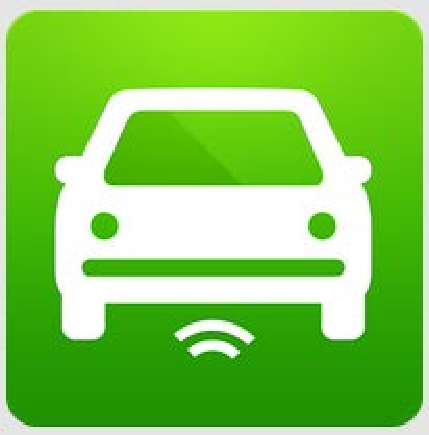
\includegraphics[scale=.6]{./estudioDeMercado/analisisDeLaOferta/source/logo_Parker}
		\caption{Logo Parker}
		\label{fig:logo_Parker}
	\end{figure}

\paragraph{Descripci�n}
Parker shows you where open parking spaces are right now in more than 30 cities and universities in the US and the UK, while also giving you access to information for over 24,000 parking lots and garages. Simply select a street with available spots or garage on the map and get turn-by-turn voice navigation. You'll also get instant access to prices, payment options, and hours.
Up to the minute parking availability is offered in Los Angeles, Hollywood, Boston, Venice Beach, Studio City, Indianapolis, Reno, Fort Lauderdale and Ellicott City MD, as well as at Clemson University and Oregon State University, with more on the way. To see a longer list, scroll below.


Features of Parker include: 
\begin{itemize}
	\item Find open parking spots, and even see on which side of the street you'll find them 
	\item Use filters to only show spots that meet your preferences. (No coins? Not a problem ? we can show you where bills or credit cards are accepted; Need accessible parking? We can show you availability for that, too.) 
	\item View prices, payment options, hours (i.e., street parking free after 7PM), and more 
	\item One touch, turn-by-turn voice navigation quickly directs you to your preferred parking location 
	\item Built-in timer reminds you when your meter is about to expire 
	\item \textit{Walk-to-Car} provides directions back to your car 
	\item View traffic conditions en route to your destination
\end{itemize}

\paragraph{Precio}
	Gratis

\paragraph{Plataformas}
	\begin{itemize}
		\item Android
	\end{itemize}
	
\paragraph{Link}
	\begin{itemize}
		\item \url{https://play.google.com/store/apps/details?id=com.streetline.parker&hl=es}
	\end{itemize}
		